%%
%% Automatically generated file from DocOnce source
%% (https://github.com/hplgit/doconce/)
%%
%%


%-------------------- begin preamble ----------------------

\documentclass[%
oneside,                 % oneside: electronic viewing, twoside: printing
final,                   % draft: marks overfull hboxes, figures with paths
10pt]{article}

\listfiles               %  print all files needed to compile this document


\usepackage[totoc]{idxlayout}   % for index in the toc
\usepackage[nottoc]{tocbibind}  % for references/bibliography in the toc

\usepackage{relsize,makeidx,color,setspace,amsmath,amsfonts,amssymb}
\usepackage[table]{xcolor}
\usepackage{bm,ltablex,microtype}
\usepackage{comment} 
\usepackage[pdftex]{graphicx}

\usepackage{fancyvrb} % packages needed for verbatim environments

\usepackage[T1]{fontenc}
%\usepackage[latin1]{inputenc}
\usepackage{ucs}
\usepackage[utf8x]{inputenc}

\usepackage{lmodern}         % Latin Modern fonts derived from Computer Modern

% Hyperlinks in PDF:
\definecolor{linkcolor}{rgb}{0,0,0.4}
\usepackage{hyperref}
\hypersetup{
    breaklinks=true,
    colorlinks=true,
    linkcolor=linkcolor,
    urlcolor=linkcolor,
    citecolor=black,
    filecolor=black,
    %filecolor=blue,
    pdfmenubar=true,
    pdftoolbar=true,
    bookmarksdepth=3   % Uncomment (and tweak) for PDF bookmarks with more levels than the TOC
    }
%\hyperbaseurl{}   % hyperlinks are relative to this root

\setcounter{tocdepth}{2}  % levels in table of contents

% --- fancyhdr package for fancy headers ---
\usepackage{fancyhdr}
\fancyhf{} % sets both header and footer to nothing
\renewcommand{\headrulewidth}{0pt}
\fancyfoot[LE,RO]{\thepage}
% Ensure copyright on titlepage (article style) and chapter pages (book style)
\fancypagestyle{plain}{
  \fancyhf{}
  \fancyfoot[C]{{\footnotesize \copyright\ 1999-2018, "Computational Physics I FYS3150/FYS4150":"http://www.uio.no/studier/emner/matnat/fys/FYS3150/index-eng.html". Released under CC Attribution-NonCommercial 4.0 license}}
%  \renewcommand{\footrulewidth}{0mm}
  \renewcommand{\headrulewidth}{0mm}
}
% Ensure copyright on titlepages with \thispagestyle{empty}
\fancypagestyle{empty}{
  \fancyhf{}
  \fancyfoot[C]{{ }}
  \renewcommand{\footrulewidth}{0mm}
  \renewcommand{\headrulewidth}{0mm}
}

\pagestyle{fancy}


% prevent orhpans and widows
\clubpenalty = 10000
\widowpenalty = 10000

% --- end of standard preamble for documents ---


% insert custom LaTeX commands...

\raggedbottom
\makeindex
\usepackage[totoc]{idxlayout}   % for index in the toc
\usepackage[nottoc]{tocbibind}  % for references/bibliography in the toc
\usepackage{listings}
\usepackage[normalem]{ulem} 	%for tables
\useunder{\uline}{\ul}{}
\usepackage{hyperref}
\usepackage[section]{placeins} %force figs in section

%-------------------- end preamble ----------------------

\begin{document}

% matching end for #ifdef PREAMBLE

\newcommand{\exercisesection}[1]{\subsection*{#1}}


% ------------------- main content ----------------------



% ----------------- title -------------------------

\thispagestyle{empty}

\begin{center}
{\LARGE\bf
\begin{spacing}{1.25}
Simulating the Solar System using ordinary differential equations
\end{spacing}
}
\end{center}

% ----------------- author(s) -------------------------

\begin{center}
{\bf Noah Oldfield and Johan Nereng}
\end{center}

    \begin{center}
% List of all institutions:
\centerline{{\small Department of Physics, University of Oslo, Norway}}
\end{center}
    
% ----------------- end author(s) -------------------------

% --- begin date ---
\begin{center}
Sep 8, 2018
\end{center}
% --- end date ---

\vspace{1cm}

\section{Introduction}
ØK MARGINEN!


\textbf{Legg till litt mer om motivasjon for prosjektet} \newline
The overall aim of this project is to develop a program that simulates the Solar System by numerically solving equations that describe the trajectory of the planets and the Sun. The motion of each of these objects is subject to the sum of forces acting upon that object, and it's trajectory may be described through a set of coupled ordinary differential equations (ODEs). \newline



. \newline
First, choice of numerical procedure (for solving the ODEs) is decided upon, empathizing run time and stability. In this project, both the velocity Verlet and Forward Euler method (\hyperref[sec:NPs]{here}) were evaluated - upon which the velocity verlet was decided upon as the most suitable method due to \textbf{kort beskrivelse av hvorfor Verlet ble valgt}\newline

After describing the procedures, algorithms using both methods were developed (\hyperref[sec:NPalgo]{here}). \newline

Having developed algorithms, both algorithms were tested in a prototype program using a simplified version of the Solar System, described in detail \hyperref[sec:NPalgo]{here}.


All sims run over one year, except last stuff

I Intro: all data er henta fra NASA, med dato: posisjoner 20.oktober 2017 (for å kunne sammenlignde med årets pos)


1. Finn metode for simulering (Sun/Earth)
2. Implementer generell M-body algoritme (solsystemet)
3. Simuler hele solsystemet
4. Hva med relativitet?

assumes general understanding of forces, and the sum of forces on an object.
\section{Methods}

\subsection{Numerical procedures for solving ODEs}
\label{sec:NPs}
The procedures \cite{HJ-ODE} described in this section are general numerical solvers for ordinary differential equations. This means that the procedures assumes that the problem at hand is properly discretized.  Throughout this project, all discretization is carried out using the same template. The specific discretization paramters for each particular system is described in more detail later.  \newline

\subsubsection*{Discretization template}
Time, $t$ - running from an initial value $t_0$ to $t=T$,  is discretized over $n$ points with a step length $h=1/(n-1)$, so that $t_i=t_0 + ih$, where $i=0,1,...,n-1$. $x_i$, $v_i$ denotes position and velocity (in the $x$ direction) at time $t_i$, and $\frac{d^2x_i}{dt_i^2}=f(x_i,t_i)$ denotes the discretized second derivative of position - or the acceleration. Same procedure for $y$ and $z$ direction.

\subsubsection{Euler’s Forward method}
\begin{align*}
x_{i+1}&=x_i+hv_{i}\\
v_{i+1}&=v_{i}+hf(x_i,t_i)\\
\end{align*}
For the Euler's Forward method method, the local truncation error (LTE) is $O(h)=h^2$.
\newline
\subsubsection{Velocity Verlet method}
When using the Velocity Verlet method, $x_{i+1}$ must be determined before $v_{i+1}$ as $f(x_{i+1},t_{i+1})$ depends on $x_{i+1}$.
\begin{align*}
x_{i+1}&=x_i+hv_{i}+\frac{h^2}{2}f(x_i,t_i) \\
v_{i+1}&=v_{i}+\frac{h}{2} \big(f(x_{i+1},t_{i+1})+f(x_i,t_i) \big) \\
\end{align*}
For the Velocity Verlet method method, the local truncation error (LTE) is $O(h)=h^3$.


\subsection{Developing algorithms}
\label{sec:NPalgo}
Before applying the numerical procedures to a particular system, an algorithm for each method is first developed. The algorithms use non-specific parameters, which ensures flexibility in implementation (choice of system). The algorithms does however assume that the acceleration of an object at time $t$ depends on the mass of the object and the state of the system at time $t$ . \newline 
In order to evaluate the algorithm implementations, a specific system must be decided upon, which also fixes the number of floating point operations.  

\subsubsection*{On facilitating implementation to code}
In order to later develop effective and transparent code, the use vectorization is assumed. This means that $\vec{r}=(x,y,z)$, $\vec{v}=(v,u,w)$ contains the position and velocity components in the $x,y,z$ direction. Similarly, derivatives and forces are assumed to be three dimensional.  \newline

\subsubsection*{The algorithms}
\label{subsec:algos}
The following algorithms approximates the position $r_j=(x_j(t),v_j(t),z_j(t))$ and velocity $v_j=(v_j(t),u_j(t),w_j(t))$ in three dimensions for $1,2,..,j,...,M$ objects with mass $m_j$ at time $t_1, t_2,..,t_{n-1}$, provided that the the initial values are known. In addition, the algorithm assumes that the acceleration at a given time $t$ of object $j$ depends on the current state of the system, and the mass of the object itself - that is: $a_j=f(t,m_j)$. The algorithms overwrites $r_j$ and $v_j$ at every time step. \newline

The Euler's forward algorithm below has floating point operations: \newline
\# flops$\sim n \cdot (1+j \cdot (4+\text{(\#flops in } a_j))$

\begin{center}\fbox{\parbox{\textwidth}{{\textbf{Algorithm for solving $3$ dimensional $M$ body system using Euler's forward method}}
\begin{enumerate}
\item \textbf{Calculate} $h=1/(n-1)$
\item \textbf{For} $j = 1,2,..,M$:
\subitem \textbf{Initialize} vectors: $r_j$, $v_j$ and $a_j$ with dimension $3$.
\subitem \textbf{Set} $m_j$
\subitem \textbf{Set} $r_j$ and $v_j$ to initial values.
\item \textbf{Set} $t=0$
\item \textbf{For} $i =1,2,...,(n-1)$:
\subitem \textbf{For} $j = 1,2,..,M$:
\subsubitem \textbf{Update:} $a_j=f(r_j,m_j)$
\subitem \textbf{For} $j = 1,2,..,M$:
\subsubitem \textbf{Update:} 
\subsubitem $r_j=r_j+hv_{j}$
\subsubitem $v_j=v_{j}+ha_j$
\subitem \textbf{Update} $t=t+h$
\end{enumerate}}}\end{center}

As mentioned under \hyperref[sec:NPs]{Numerical procedures for solving ODEs}, the velocity Verlet method (algorithm below) makes use of the acceleration at $t_{i+1}$, $\tilde{a}_j$. Since $\tilde{a}_j=f(r_j(t_{i+1}),m_j)$, the position of all objects is updated before before $\tilde{a}_j$ is calculated. This is unproblematic as $r_j$ is not part of the expression used to update $v_j$. In order to reduce the number of floating point operations (FLOPS), $a_j$ is only calculated once (acceleration at $t_0$), and at the end of each time step, set equal to $\tilde{a}_j$. The implementation then yields that steps $1,2,3,$ and $4$ are done at $t=t_0$, while step $5$ iterates over time. \newline

The velocity Verlet algorithm below has floating point operations: \newline
\# flops$\sim n \cdot (1+j \cdot (10+2\text{(\#flops in } a_j))$, 
Which may be reduced to \# flops$\sim n \cdot (1+j \cdot (7+2\text{(\#flops in } a_j))$ by pre calculating $\frac{h^2}{2}$, and $ \frac{h}{2}$.
\begin{center}\fbox{\parbox{\textwidth}{{\textbf{Algorithm for solving $3$ dimensional $M$ body system using velocity Verlet method}}
\begin{enumerate}
\item \textbf{Calculate} $h=1/(n-1)$
\item \textbf{For} $j = 1,2,..,M$:
\subitem \textbf{Initialize} vectors: $r_j$, $v_j$, $a_j$, $\tilde{a_j}$ with dimension $3$.
\subitem \textbf{Set} $m_j$
\subitem \textbf{Set} $r_j$ and $v_j$ to initial values.
\item \textbf{Set} $t=0$
\item \textbf{For} $j = 1,2,..,M$:
\subsubitem \textbf{Update:} $a_j=f(r_j,m_j)$ (initial acceleration)
\item \textbf{For} $i =1,2,...,(n-1)$: (iterations over time start here)
\subitem \textbf{For} $j = 1,2,..,M$:
\subsubitem \textbf{Update}  $r_{j}=r_j+hv_{j}+\frac{h^2}{2}a_j$
\subitem \textbf{For} $j = 1,2,..,M$:
\subsubitem \textbf{Update:} $\tilde{a}_j=f(r_j,m_j)$
\subitem \textbf{For} $j = 1,2,..,M$:
\subsubitem \textbf{Update} $v_j=v_{j}+\frac{h}{2} \big(\tilde{a}_j+a_j) \big)$
\subsubitem \textbf{Update} $a_j=\tilde{a}_j$
\subitem \textbf{Update} $t=t+h$
\end{enumerate}}}\end{center}
  
  
  
\subsection{Sun Earth system}                                                                                                               
The first system used for algorithm implementation is the simplified model of the Solar System using only the Earth and the Sun, which constitutes a two body system. Newton's law of gravity \eqref{eq:M.SEsys.NLG} applied to the Earth with respect to the Sun  is assumed to govern the motion of the Earth, in other words - the effects of relativity is neglected. \newline


\begin{equation}
\vec{F}=\gamma \frac{M_1 M_2}{r^3}\vec{r}
\label{eq:M.SEsys.NLG}
\end{equation} 
\textit{Where $\gamma$ is a constant (usuallly $G$), $M_1$, $M_2$  the masses of two objects and $r$ the distance between their masses. In this project, all objects are assumed to be point particles} \newline


Initially, the Sun is defined as the origin, which means that $r$ is the distance to the Sun. Later, the Solar System's barycenter will be used as the origin. More on this under \hyperref[sec:Modmultibody]{The multi body system}. Assuming vector notation; $\vec{r}=(x,y,z)$ and $\vec{v}=(v,u,w)$,  Newtons law of motion: $\vec{F}=m\vec{a}$ yields: \newline
\begin{equation}
\frac{d^2 \vec{r}}{dt^2}=\frac{\vec{F}}{M_E}
\label{eq:M.SEsys.NLM}
\end{equation}

Using the Earth's mass, $M_E$ as $M_1$, and the mass of the sun $M_{\odot}$ as $M_2$, and combining \eqref{eq:M.SEsys.NLG} and \eqref{eq:M.SEsys.NLM} then leads to a system of coupled differential equations:


\begin{align}
\frac{d\vec{v} }{dt}&=-\frac{GM_{\odot}}{r^3} \vec{r} \label{eq:M.SEsys.dv/dt} \\
&\frac{d\vec{r}}{dt}=v_x \label{eq:M.SEsys.dr/dt}\\
\end{align}

Which may be discretized and solved using the methods previously discussed under \hyperref[sec:NPs]{Numerical procedures for solving ODEs}. However, prior to this, the Sun-Earth system is first scaled. 

\subsubsection{Scaling}
The following scaling will also be applied to the other systems used in this project, therefore it's written assuming that the Earth is only one of several bodies in the Solar System.\newline

Using the assumption that the trajectory of an astronomical object is (approximately) circular and in one plane, the Centripetal force may be used to scale the system. Applying one standard astronomical unit, $1 \text{ } AU$, as the length unit, and $1 \text{ } yr=1 \textit{ year}$ as the time unit, the velocity of the object may then be expressed as $v=2\pi AU/yr$. So:
\begin{equation}
GM_{\odot}=v^2r=4\pi^2  \frac{AU^3}{yr^2} 
\end{equation}
Furthermore, the Solar mass $M_{\odot}=1$ is set as the unit mass, which means that the gravitational constant is scaled as $G=4\pi^2$. This also means that the mass of an object is evaluated as a ratio of the Sun's mass. $M_E$ for example is defined as $M_E=\frac{\textit{The Earth's mass in kgs}}{\textit{The Sun's mass in kgs}}=3.0024584 \cdot  10^{-6} M_{\odot}=3.0024584 \cdot  10^{-6}$. 


\subsection{Algorithm implementation}
Having scaled and applied the discretization template discussed under \hyperref[sec:NPs]{Numerical procedures for solving ODEs} to the Sun-Earth system, the algorithms for both the Euler's Forward method and the velocity Verlet method is now implemented into code using the Sun-Earth, with the goal of developing a functioning program. This is done using $C++$ with the Vec3 class and Solar System Shell provided through the Github page of the course Computational Physics at the University of Oslo \cite{CPgithub}. The program written for the purpose of this project may be found on the authors common \href{https://github.com/johanere/CP3}{Github repository}.\newline

In order to ensure correct algorithm implementation, the initial code is written without the use of object orientation. Pending verification of successful implementation and evaluation of the numerical methods, the code will be rewritten with object orientation. More on this under \hyperref[sec:OOing]{Object orienting the code}. \newline

The code is compiled into a program using the $C++$ optimization flag $-03$ to ensure limitation of syntax discrepancies.


\subsection{Evaluation of initial implementasjon}                                                                                                                  
In order to evaluate the implementation described above, the program is first tested with $n=1000$ steps, and the results plotted for each of the two numerical methods. This is expected to produce a circular Earth orbit, bringing the Earth back to it's starting position, with some deviations due to discretization and the LTE. The velocity Verlet method is expected to produce more accurate results on account of having the smallest LTE among the two methods. \newline

A more thorough testing of the algorithm implementation is then carried out, focusing on two parameters; stability and runtime. Stability is measured through absolute error in relation to a completely circular orbit, and run time is measured by using the Chrono library from C++ - where the Euler implementation is expected to run faster than the velocity Verlet implementation, since it requires fewer FLOPS.  \newline

As the overall aim of the project is to simulate the Solar System, the code will eventually be further modified to encompass multi body systems. As multi body systems tend not to follow circular orbits, this means that comparing simulation results with a known analytical solution will eventually be infeasible. Therefore, while the absolute error is still a good measure of the stability - that is, while the program is limited to a two body system with a known solution - two alternative parameters for program stability are introduced; conservation of energy, $E$, and  conservation of angular momentum, $\omega$. By cross checking the absolute error, a well established parameter for program stability, with conservation of $E$ and $\vec{L}$, this projects seeks to establish the validity of these alternative parameters for program stability when simulating multi body systems. \newline

\subsubsection*{On conservation of Angular momentum and conservation of potential and kinetic energy}
In general, when considerer the gravitational forces acting upon  two object, each of those opposite forces acting upon one of the objects, acts in the direction of the other object. This means that the torque $\tau$ for object $1$ and $2$ may be expressed as: 

\begin{align*}
\vec{\tau}_1 =& \vec{r} \times \vec{F}_1 = 0 \\
\vec{\tau}_2 =& \vec{r} \times \vec{F}_2 = 0
\end{align*}

This, combined with the relation $\frac{d \vec{L}}{dt} = \sum_j \vec{\tau}$, implies that $\vec{L} = constant$, or that angular momentum is conserved when no external torque is acting upon the system. For a multi body system, the net force acting upon each object is the sum of forces acting upon that object. These (gravitational) forces each act in the direction of another object in the system - which again means that angular momentum is also conserved for multi body systems under the same requirements as for a two body system. \newline

The law of conservation of energy states that the total energy of an isolated system is preserved over time. Both the two body and  the multi body systems are isolated systems, and as this project does not include any energy transformations except between kinetic and potential (gravitational) energy, the sum of these quantities  is constant. \newline


\subsection{Escape velocity and effects of the gravitational force}
After having established the velocity Verlet method as better suited for the purpose of this project than the Euler's Forward method, see \hyperref[subsec:Init_implm]{Initial implementation} under discussion of results, the velocity Verlet is now further tested. This is done by evaluating the escape velocity of a planet in a two body system with the Sun.  \newline

The escape velocity, $v_{esc}$, is defined as the minimum velocity required to to escape the gravitational field of star system. This requires the planet's gravitational potential and kinetic energy to equal:
\begin{equation}
v_{esc} = \sqrt{\frac{2 G M_E}{r}}
\end{equation}

The planet's starting position is set to $1 \text{ } AU$, and it's initial velocity set to the analytical expression for $v_{esc}$ above. If the potential energy at any point is great that the kinetic energy however, the planet will not escape the Sun's gravitational field. As the program uses several simplifications and is a numerical solver, the planet is not expected to escape. Therefore, by tial and error, different initial velocities are tested in order to find a more representative $v_{esc}$ for the simulated system.\newline

In addition, in order to evaluate the effects of the gravitational force, the force is modified \eqref{eq:M.gravmod} and the code rerun, using the Sun-Earth system.
\begin{equation}
F_G=\frac{GM_{cdot}M_{E}}{r^{\beta}}
\label{eq:M.gravmod}
\end{equation}
Where $\beta \in [2,3]$ is tested, empathizing the effects on the Earth-Sun system when $lim_{\beta} \rightarrow 3$.

 
\subsection{Object orienting the code}  
\label{sec:OOing}
Using object oriented code with C++, the algorithm implementation of the velocity Verlet on the two body system is modified in order to obtain modularity, re-usability and polymorphism.  \newline

As the specific C++ syntax applied may be found under on the authors common \href{https://github.com/johanere/CP3}{Github repository}, this section only includes a brief description of the overall train of thought in the object orientation process. \newline

First, a (solar) system class is defined, to which planets may be added, as well as a trajectory governing force (gravity). Other objects than planets may also be added, as the system only serves to store the objects that are a part of the system, not their types. In addition, other governing forces than gravity may be defined. This is utilized later, when \hyperref[sec:M.effectsofrel]{the effects of relativity} on the simulation are explored. The system class also includes a method to reset the forces at each time step\newline

As this project only makes use objects of the same type (planets), a celestial bodies class is defined in order to facilitate the simulation of an $M>2$ body system. By defining the celestial bodies to store $\vec{r}$ and $\vec{v}$ at the current time, $m$, and the name of each celestial body, any number of objects may be added to the system. The force (class) is set up in a way that enables it to calculate all forces between objects at their current position - $\tilde{a}$ in the velocity Verlet algorithm. \newline

Lastly, a solver class is defined - which upon construction is supplied with a specific system. The solver serves to advance that system from $t_{0}$ to $T$, by iterating over $n$ time steps. This is done by calling a numerical procedure specific function, taking $n$ as an argument. In this project, the velocty Verlet method is implemented, but other methods may be defined for the solver. The velocity Verlet \hyperref[subsec:algos]{algorithm} is (almost) directly implemented, as it was devloped in order to encompass multi body systems. \newline

In order to verify the integrity of the algorithm, a simple simulation of the Sun-Earth system is carried out by using $n=1000$. This is expected to produce a plot similar to the one produced under initial testing (of the velocity Verlet algorithm).


\subsection{NASA data and system barycenter}
As the focus of this project now shifts from the simplified Solar System model using only the Earth and the Sun, to a model containing three, then all planets, initial positions and velocities of the objects are expected to approximate actual values. To accomlish this, ephemerides for the relevant Solar System bodies are extracted from the limited interface to JPL's HORIZONS system provided by NASA \cite{nasadata}, in $AU$. These ephemerides use the Solar System's barycenter as the origin, which means that the Sun is no longer fixed at the origin - this is described further in the discussion of results section under  \hyperref[subsec:Discofres:3B]{the three body system}.  \newline

Masses and velocities are also extracted from the HORIZONS system interface and scaled to fit unit's of measurements used in this project.

\subsection{Three body system}
\label{sec:Modmultibody}
The final step before simulating the Solar System with all planets, is to test the object oriented code using a three body system. This is carried out by adding the Sun, the Earth, and Jupiter to the system class, using HORIZONS system data as described above. The system is solved using the velocity Verlet function from the Solver class on a selection of $n$ \textbf{WHAT VALUES?}, and the stability of the solution is evaluated by conservation of angular momentum, which is established as a suitable stability measurement in the discussion of results section under \hyperref[subsec:Discofres:initimpl]{Inital implementation}. \newline

After initial stability testing of the Sun-Earth-Jupiter system using the object oriented code, the mass of Jupiter, $M_J$ is increased. First by a factor of $10^1$, then by $10^3$. This is expected to have an effect on the trajectory of all three bodies; on the Sun - a pronounced trajectory, on Jupiter - a pronounced trajectory, and on the Earth - \textbf{SOMETHING??}. Especially in the $M_J=10^3 M_J$ case. First, stability tests are executed for each case, then plots are produced, visualizing the effect on the system.
  
\subsection{Simulating the Solar System}
After having established the integrity of the applied simulation methods for multi body systems under discussion of results (\hyperref[subsec:Discofres:3B]{the three body system}), the Solar System is now simulated using all $8$ planets and the Sun. All $9$ objects are initialized using HORIZONS system data. Then, using $n=$ - established as suitably stable for the multi body system implementation under discussion of results, the program is executed and the results plotted. \textbf{NOE MER?}

 
\subsection{Effects of relativity}
\label{sec:M.effectsofrel}
As previously mentioned, the Solar System model simulation developed in this project does not include the effects of relativity. In order to address this discrepancy, the noe of mercus is now examined.
 4. Kjør Sol og merkur
- Aphelion/Perihelion beskrive ( og vinkel perihelion)
- Forklar generell relativitet ledd i kraft

\section{Results}
\subsection{Testing of initial implementation}
flops - euler faster as expected?

Figure \ref{fig:twobodyplot} shows....

\begin{figure}[!htb]
        \centering 
         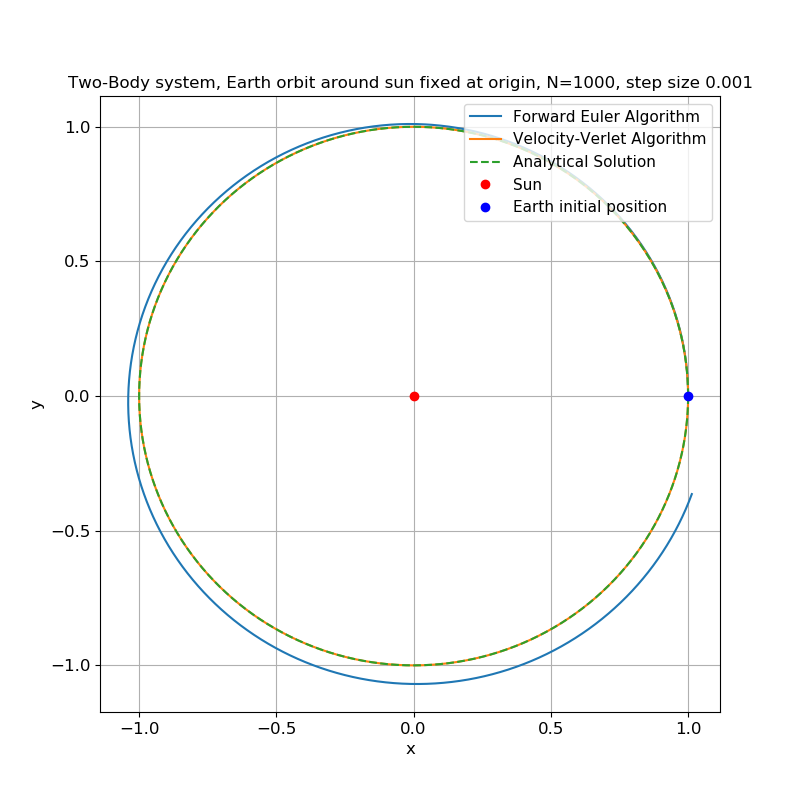
\includegraphics[scale=.6]{../Results/twoBodyNOOplot1.png} 
        \caption{Plot of numerical solutions of the two body system: Sun-Earth, generated by the Euler's Forward and the velocity Verlet method}
        \label{fig:twobodyplot}   
\end{figure}  

 Initiell sjekk av at simuleringa fungerer som forventa: plot med sol jord, se at sirukær bane. 
    - Kommenter: hva ser vi her?
1.2 Tabell (ved sirkulær bane, to object, sun fixed) Euler og Verlet:
    - N, Runtime, max abs error for 1 år, største avvik energi avvik fra energi ved $t_0$, og tilsv for $angmom_tot $
    - Kommenter: hva ser vi her?
    
 -----KUN VERLET HERFRA -------

\subsection{Object Orientation: verifying integrity of methods} Plot med sol og jord, sun fixed som viser at simuleringa fortsatt fungerer
 
\subsection{Escape velocity}
1.3 $(V_esc)$ Presenter plot med analytisk $v_esc.$ Deretter $v_esc$ ved trial and error. Kommenter forskjell (høyere eller lavere enn analytisk?)
\subsection{Effects of gravitational force}
1.4 (Tyngekrafta)  Multiplot med bane for sol jord med ulike beta

\subsection{Multi Body: Verifying integrity of implementation }
2.1 - Plot ESJ oppå ES
    - For en N som tidligere har vært stabil - presenter momentumbevaring. Samme toleranse? Må vi øke N for samme stabilitet?
\subsection{Multi Body: The effects of another object on the Earth's trajectory}
    - plot for jupmassse x10 og x1000

\subsection{Solar System:verifying integrity of implementation }
- Plot over solsystemet for ett år <- simuleringa fungerer som forventa
- Stabilitetssjekk: Angmom bevart? 

\subsection{Effects of relativity}
4. Kjør Sol (flytende sol) og merkur 
- finn vinkel etter 100 år med newtonsk
- finn vinkel etter 100 år med generell relativitet

\section{Discussion of results}

\subsection{Initial implementation}
\label{subsec:Discofres:initimpl}
floats - same $a$ -> verlet has more floats, should take longer
\label{subsec:Init_implm}
 Ser ut til at simuleringa fungerer
1.2 Verlet er bedre
 -----KUN VERLET HERFRA -------
 
Since both angular momentum and the sum of potential and kinetic energy should be preserved for any isolated multi body system, either parameter should be a valid measure of program stability, both for a two body system and for a multi body system. Table .... strengthens this hypothesis. As both paramters have .... , conservartion of angular momentum is chosen for all stability evaluations in the rest... numeriske metoder kan ødelegge bevaringa - antall punkter,metode.
 
 
\subsection{Escape velocity}
1.3 $(V_esc)$ Er det en sammenheng med hva vi så på energibevaring elns? 
\subsection{Effects og gravitational force}
1.4 (Tyngekrafta) Kommenter noe på beta-> med høyere beta, avtar tyngekrafta fortere med avstand -> planetene stikekr av

\subsection{The three body system}
\label{subsec:Discofres:3B}
As the data from NASA uses a barycenter that includes objects that are not in use in this project, the barycenter may be 
barycenter - include bodies not used in our simulating - may have effects on solution.
\subsubsection{Integrity of methods}
-Verlet funker med 3 bodies
- se at jordas bane (og solas) blir i økende grav påvirka.
\subsubsection{Effects on Earth's trajectory}

\subsection{Solar system}
\subsubsection{Integrity of methods}
- Ser plottet ut som forventa? Noen planeter ikke fullført bane -> de bruker lengre tid enn 1 yr!
- Stabilitetssjekk: Angmom bevart ved en viss N med lik nøyaktighet som før?

- sucessfully simulated a simplified version of the solar system using all planets and newtonian gravity - not accounted for relativty and other astronomical objects 
\subsection{Effects of relativty}
beskriv avviket på vinkel. Er det viktig å ta med generell relativitet?
\section{Conclusions}

\bibliographystyle{plain}
\bibliography{ref}


\end{document}





% ------------------- end of main content ---------------



